\documentclass[a4paper,landscape]{article}
\usepackage[margin=1in]{geometry}
\usepackage{graphicx}
\usepackage{xcolor}
\usepackage{tikz}
\usetikzlibrary{decorations.pathmorphing,calc}
\usepackage{newtxtext}
\usepackage{newtxmath}
\renewcommand{\familydefault}{\sfdefault}
\pagenumbering{gobble}
\usepackage{ragged2e}
\usepackage{eso-pic}

% Put full-page background if present
\AddToShipoutPictureBG*{
  \AtPageLowerLeft{%
    
\includegraphics[width=\paperwidth,height=\paperheight]{background.png}%
  }
}

\begin{document}
\thispagestyle{empty}

% central faint watermark logo (if logo.png exists)
\begin{tikzpicture}[remember picture, overlay]
  \node[anchor=center, opacity=0.08] at (current page.center) {
    
\includegraphics[width=0.55\paperwidth,keepaspectratio]{logo.png}
  };
\end{tikzpicture}

% Header: top-left and top-right monk logos and institute/title text
\begin{tikzpicture}[remember picture, overlay]
  % left monk
  \node[anchor=north west, yshift=-0.8cm, xshift=1.5cm] at (current page.north west)
    {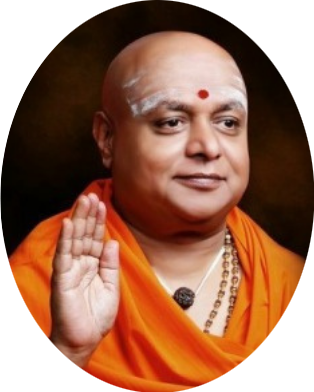
\includegraphics[height=3.5cm]{Swamiji1-modified.png}};
  % right monk
  \node[anchor=north east, yshift=-0.8cm, xshift=-1.5cm] at (current page.north east)
    {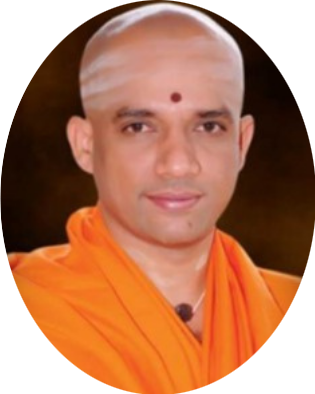
\includegraphics[height=3.5cm]{Swamiji2-modified.png}};

  % center institute text
  \node[align=center, anchor=north] at ([yshift=-0.8cm]current page.north) {
    {\fontsize{12}{12}\selectfont \textbf{|| JAI SRI GURUDEV ||}}\\[0.2cm]
    {\fontsize{16}{18}\selectfont \textbf{ADICHUNCHANAGIRI INSTITUTE OF TECHNOLOGY}}\\[0.1cm]
    {\fontsize{11}{13}\selectfont \textbf{JYOTHI NAGARA, CHIKKAMAGALURU-577102, KARNATAKA, INDIA}}\\[0.1cm]
    {\fontsize{13}{14}\selectfont \textbf{DEPARTMENT OF COMPUTER SCIENCE \& ENGINEERING}}
  };
\end{tikzpicture}

% Big certificate heading
\begin{center}
  \vspace*{2.5cm}
  {\fontsize{48}{48}\selectfont\textbf{CERTIFICATE}}\\[0.2cm]
  {\fontsize{20}{22}\selectfont\textbf{OF PARTICIPATION}}\\[1.2cm]
  {\fontsize{20}{24}\selectfont This is to certify that}\\[0.8cm]
  {\fontsize{28}{30}\selectfont \textbf{__PARTICIPANT__}}\\[0.6cm]
  {\fontsize{14}{18}\selectfont \textbf{Team:} \underline{\textbf{__TEAM__}}}\\[0.9cm]
  {\fontsize{14}{18}\selectfont This is to certify that the above participant has taken part in HACKABHIGNA (domain name), a 24-Hours National-Level Hackathon organized by the Department of Computer Science \& Engineering, Adichunchanagiri Institute of Technology.}\\[1.2cm]
\end{center}

% Sponsor / collaborator logos and labels
\begin{tikzpicture}[remember picture, overlay]
  \node[anchor=north, yshift=-9.8cm] at (current page.north) {
    \begin{minipage}{0.8\textwidth}
      \centering
      {\fontsize{14}{16}\selectfont \textbf{In Collaboration with}}\\[0.25cm]
      
\includegraphics[height=0.7cm]{google gemini logo.png}\hspace{1cm}
      
\includegraphics[height=0.7cm]{streamz.png}\hspace{1cm}
      
\includegraphics[height=0.7cm]{environ.jpg}\\[0.4cm]
    \end{minipage}
  };
  % Knowledge partner at right
  \node[anchor=north east, yshift=-9.8cm, xshift=-1.5cm] at (current page.north east) {
    \begin{minipage}{3cm}\centering
      {\fontsize{12}{12}\selectfont \textbf{Knowledge Partner}}\\[0.1cm]
      
\includegraphics[height=0.8cm]{ICT.png}
    \end{minipage}
  };
\end{tikzpicture}

% Signatures row at bottom
\begin{tikzpicture}[remember picture, overlay]
  \node[anchor=south, yshift=2.3cm] at (current page.south) {
    \begin{minipage}{0.9\textwidth}
      \centering
      \begin{tabular}{ccc}
        \begin{minipage}{0.28\textwidth}\centering
          \rule{6cm}{0.4pt}\\[0.2cm]
          \textbf{Dr. Pushpa Ravikumar}\\
          Professor & Head, Dept. of CS\&E\\
          AIT, Chikkamagaluru
        \end{minipage} &
        \begin{minipage}{0.28\textwidth}\centering
          \rule{6cm}{0.4pt}\\[0.2cm]
          \textbf{Dr. C. T Jayadeva}\\
          Principal\\
          AIT, Chikkamagaluru
        \end{minipage} &
        \begin{minipage}{0.28\textwidth}\centering
          \rule{6cm}{0.4pt}\\[0.2cm]
          \textbf{Dr. C. K Subbaraya}\\
          Director, AIT \\ Register, ACU
        \end{minipage}
      \end{tabular}
    \end{minipage}
  };
\end{tikzpicture}

\end{document}
